\documentclass[11pt]{article}
\usepackage{setspace}
\usepackage[a4paper,margin=1in]{geometry}
\geometry{margin=0.85in}
\setstretch{1.0}
\usepackage{graphicx}
\usepackage{array}
\usepackage{setspace}
\usepackage{parskip}
\usepackage{ragged2e}

\pagestyle{empty}
\setstretch{1.0}

\begin{document}


% Title
\begin{center}
    {\Large \textbf{Job Application}} \\[3cm]
    
    {\Huge \textbf{Zhongli Wang}} \\[0.4cm]
    
    {\huge Application for Quantitative Research Internship}
\end{center}

\vspace{0.6cm}

% Large picture in the middle
\begin{center}
    \IfFileExists{../zhongli-wang-profile.jpg}{
        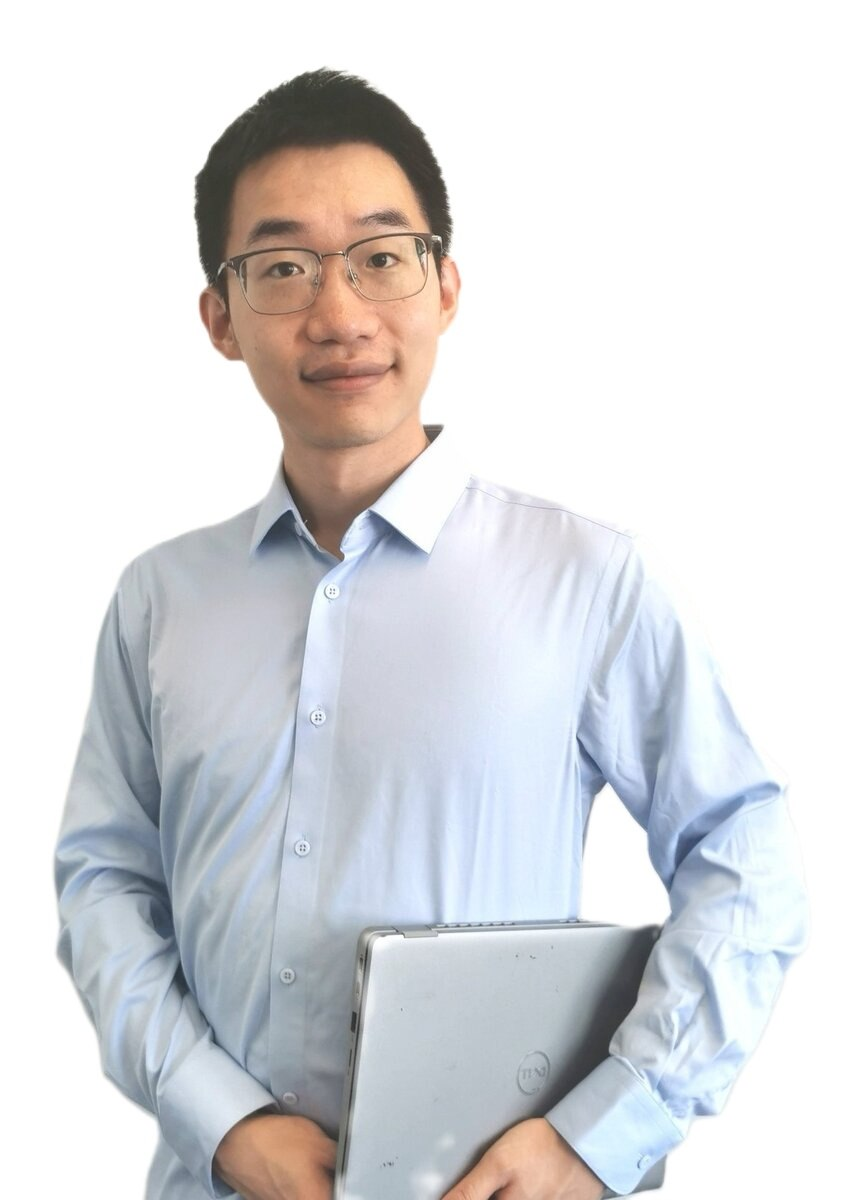
\includegraphics[
            width=0.55\textwidth,
            height=0.45\textheight,
            keepaspectratio
        ]{../zhongli-wang-profile.jpg}
    }{
        \vspace{0.45\textheight}
    }
\end{center}

\vspace{0.7cm}

% \vspace{3cm}


% Personal details
\begin{center}
\renewcommand{\arraystretch}{1.35}
\begin{tabular}{>{\bfseries}p{4.2cm} p{8.5cm}}


Address: & Astastrasse 22, 33617 Bielefeld, Germany \\

Number: & +49 160 9541 6015 \\

Email: & nkwangzhongli@gmail.com \\
\end{tabular}
\end{center}

\vfill

% \begin{center}
%     \small Last updated: \today
% \end{center}
\newpage
\enlargethispage{4\baselineskip}

\begin{flushright}
Zhongli Wang \\
Astastrasse 22 \\
33617 Bielefeld \\
Germany \\
\end{flushright}

\vspace{0.1cm}

\noindent
One Island East 57th Fl \\
18 Westlands Rd \\
Taikoo Place \\
Hong Kong

\vspace{0.1cm}

\noindent
Application for Quantitative Research Internship - PhD: Summer 2027 at Susquehanna \\

\vspace{0.05cm}

\noindent Dear Susquehanna Hiring Team,

I am writing to apply for Susquehanna's Quantitative Research Internship - PhD: Summer 2027. 
I am completing the final stage of my Ph.D. in Economics at Bielefeld University, with my defense scheduled for September 21, 2026, 
and I also hold an M.A. in Business and Economics with a Banking and Finance major and a B.Sc. in Finance. 
My training connects statistical modeling, machine learning, financial data analysis, and computational models of strategic behavior, 
which fits the internship's focus on turning data into testable alphas.

Susquehanna is attractive to me because the program combines modeling, execution, evaluation, education, and open collaboration. 
That mirrors how I work: form a hypothesis, implement it in code, test it against data, inspect failure cases, and revise. 
I understand the internship is U.S.-based with full-time placement in Hong Kong upon graduation, and Hong Kong is one of my target long-term locations.

My closest fit with the role is the ability to connect quantitative reasoning with careful empirical execution. 
In my doctoral work, I build computational models of competing firms, estimate parameters, and analyze how network effects, capacity limits, and market structure change outcomes under uncertainty. 
In a published financial fraud detection project, I used accounting, financial, and market indicators with XGBoost to identify red flags in listed companies.

I would bring the following strengths to Susquehanna's quantitative research team:

\begin{itemize}
    \item \textbf{Research discipline:} Econometrics, machine learning, SMM, MCMC, and agent-based modeling applied to noisy, competitive environments.
    \item \textbf{Python data analysis:} Advanced Python for modeling and machine learning, with R, Julia, Mathematica, SQL foundations, Git, and reproducible workflows.
    \item \textbf{Strategic reasoning:} Research on strategic firm behavior, network effects, and capacity constraints, plus training in quantitative finance and financial engineering.
\end{itemize}

At Susquehanna, I would aim to contribute through clean research pipelines, disciplined backtests, 
and careful analysis of when a signal is robust, regime-dependent, or not useful. 
I am self-motivated, quick to learn, and comfortable presenting model assumptions, validation choices, and empirical results under scrutiny.

Thank you for your time and consideration. 
I would welcome the opportunity to discuss how my research background, financial training, 
and coding experience can contribute to Susquehanna's Quantitative Research Internship program.

\vspace{0.05cm}
\noindent Sincerely, \\[0.08cm]
\noindent Zhongli Wang \\[-0.2cm]

\vspace{0.1cm}
\noindent
\includegraphics[width=2.7cm,keepaspectratio]{../Wang-sig.jpg}

\end{document}
